\documentclass[12pt,letterpaper]{article}

% ── Packages ──────────────────────────────────────────────────────────────────
\usepackage[margin=1in]{geometry}
\usepackage{setspace}\doublespacing
\usepackage{amsmath,amssymb}
\usepackage{graphicx}
\usepackage{booktabs}
\usepackage{natbib}
\usepackage{hyperref}
\usepackage{xcolor}
\usepackage{caption}
\usepackage{subcaption}
\usepackage{tabularx}
\usepackage{float}

\hypersetup{colorlinks=true,linkcolor=blue!60!black,citecolor=blue!60!black,urlcolor=blue!60!black}
\bibliographystyle{aer}

% ── Title ─────────────────────────────────────────────────────────────────────
\title{\textbf{Identifying Directed Belief Propagation\\in Macro Prediction Markets}}
\author{Haotian Yang\thanks{BEMACS, Bocconi University. Email: \href{mailto:haotian.yang@studbocconi.it}{haotian.yang@studbocconi.it}. I thank Marco Ottaviani, Eric Zitzewitz, and Lin Peng for valuable comments. All errors are my own.}}
\date{\today}

\begin{document}
\maketitle
\thispagestyle{empty}

% ══════════════════════════════════════════════════════════════════════════════
% ABSTRACT
% ══════════════════════════════════════════════════════════════════════════════

\begin{abstract}
\noindent How do market beliefs about macroeconomic events influence each other? We construct a directed network of 19 macro prediction market composites on Kalshi---spanning monetary policy, inflation, fiscal risk, trade, and political outcomes---and use scheduled announcements (FOMC, CPI, NFP) as natural experiments to separate genuine cross-category information flow from differential-speed reactions to common shocks. Three independent identification strategies converge: event-window decomposition classifies edges by their behavior around macro announcements, FOMC event-studies isolate anticipatory versus reactive price dynamics, and lead-lag asymmetry tests distinguish directed flow from symmetric co-movement. Of 176 unique directed edges, 62\% reflect genuine information channels; only 3.4\% are common-shock artifacts---an order of magnitude below the $>$80\% contamination rate documented in equity networks \citep{yang2026te}. The identified network reveals three structural features invisible without identification: (i)~FOMC internal dynamics---not rate decisions themselves---are the primary information originator across all macro categories; (ii)~tariff expectations function as an information relay, absorbing monetary and fiscal signals and retransmitting them to political contract categories; (iii)~government shutdown risk is the dominant source of fiscal information, whose effect on growth expectations is fully mediated by the tariff relay---revealing tariffs as the central transmission hub of the macro belief network. These findings demonstrate that prediction markets provide a setting where directed financial network edges have clean economic interpretation---and where the identification problem that plagues equity network estimation can be solved.

\medskip
\noindent\textit{JEL Codes:} G14, G17, E44, C32, D83\\
\textit{Keywords:} prediction markets, information networks, identification, macro beliefs, directed information flow
\end{abstract}

\newpage
\setcounter{page}{1}

% ══════════════════════════════════════════════════════════════════════════════
% 1. INTRODUCTION
% ══════════════════════════════════════════════════════════════════════════════

\section{Introduction}

On September 17, 2025, the Federal Reserve announced a rate hold at 4.25--4.50\%, accompanied by two dissenting votes favoring an immediate cut. Within hours, Kalshi prediction markets registered a cascade of price adjustments: not only in contracts directly referencing the Fed Funds rate, but in inflation expectations, government shutdown probabilities, GDP growth forecasts, and even congressional policy narratives. Some contracts moved within minutes; others adjusted gradually over days. Which of these cross-contract price dynamics reflect genuine information transmission---the Fed's internal disagreement revealing something new about inflation or growth---and which are simply different contracts reacting to the same public announcement at different speeds?

This question---what fraction of observed directed relationships in financial networks are genuine information channels versus artifacts of differential response to common shocks---has no answer in the existing literature. The financial network estimation literature, launched by \citet{billio2012econometric} and extended by the \citet{diebold2014network} connectedness framework, has produced hundreds of directed network studies in equity, credit, and macro-financial settings. These studies treat statistically significant edges as meaningful predictive relationships. Yet none asks the identification question: when contract~A's price history predicts contract~B's future price, is this because A carries information relevant to B, or because both respond to the same shock and A happens to adjust faster? The theoretical mechanism for this confound is well established. \citet{ottaviani2015price} show that in markets with heterogeneous prior beliefs, prices underreact to public information at rates determined by the trader population's belief dispersion. When a common shock hits two markets, differential underreaction speeds generate the appearance of directed information flow---a statistical artifact with no economic content.

We propose the first systematic identification framework for directed information flow in financial networks. Our setting is the Kalshi prediction market, where 4,003 macro event contracts are collapsed into 19 composite nodes spanning monetary policy, inflation, growth, fiscal risk, trade, and political outcomes. Three features of this setting enable identification that is impossible in equity markets: contract prices are named event probabilities with clean semantic interpretation, the number of nodes is naturally small ($N=19$, keeping estimation in reliable regimes), and scheduled macroeconomic announcements---18 FOMC decisions, 26 CPI releases, 26 NFP reports---provide exogenous information shocks with known timing, functioning as natural experiments for edge decomposition.

Our identification framework deploys three independent strategies that converge on a unified edge classification. Event-window decomposition splits rolling estimation windows by macro announcement density and classifies each edge by whether it appears in high-event periods, quiet periods, or both. FOMC event-studies examine the temporal dynamics of each edge around Federal Reserve announcements, distinguishing anticipatory information leaders from post-announcement common-shock responders. Lead-lag asymmetry tests measure the directionality of each edge pair, separating genuine one-directional flow from symmetric co-movement suggestive of common factors. The triangulation of these three methods---each exploiting different variation in the data---provides robust classification without relying on any single test.

The identified network reveals three structural features that are invisible in the raw network. First, FOMC internal dynamics---disagreement among committee members, leadership transitions, communication about future policy paths---are the primary information originator across all macro categories, ranking above the Fed Funds rate level itself in the information hierarchy. Second, global tariff expectations function as an information relay node, absorbing signals from monetary and fiscal contracts and retransmitting them to political and trade policy categories. Third, government shutdown risk is the dominant source of fiscal information, but its effect on growth expectations is fully mediated by the tariff relay---conditional analysis shows the direct shutdown-to-growth edge vanishes when tariffs are controlled for, while both segments of the indirect pathway (\texttt{gov\_shutdown} $\to$ \texttt{global\_tariffs} $\to$ \texttt{gdp}) survive, revealing tariffs as the central transmission hub of the macro belief network.

We contribute to three literatures. To the financial network estimation literature \citep{billio2012econometric,diebold2014network,barigozzi2019nets}, we provide the first identification framework that decomposes directed edges into genuine information flow versus common-shock artifacts, demonstrating that prediction markets---where the identification problem is solvable---serve as a calibration benchmark for the contamination rates that plague equity networks. To the prediction market literature \citep{wolfers2004prediction,snowberg2013prediction,bergemann2021information}, we introduce a cross-contract network perspective that reveals how information propagates across event categories, filling a gap identified by \citet{bergemann2021information} who note the absence of cross-market information dynamics. To the macro-finance literature on information transmission \citep{gurkaynak2005actions,bauer2023alternative}, we provide a data-driven directed map of how macro beliefs interact, complementing the event-study tradition with a continuous network perspective.

The remainder of the paper is organized as follows. Section~\ref{sec:data} describes the data and network construction. Section~\ref{sec:identification} presents the identification framework. Section~\ref{sec:results} reports the main findings. Section~\ref{sec:robustness} provides robustness checks. Section~\ref{sec:conclusion} concludes.

% ══════════════════════════════════════════════════════════════════════════════
% 2. DATA AND NETWORK CONSTRUCTION
% ══════════════════════════════════════════════════════════════════════════════

\section{Data and Network Construction}\label{sec:data}

\subsection{Kalshi Prediction Markets and Composite Construction}

Kalshi is a CFTC-regulated event contract exchange where each contract pays \$1 if a specified event occurs and \$0 otherwise. Contract prices, quoted in cents from 0 to 100, are directly interpretable as market-implied event probabilities. We collect 4-hour candlestick data for 2,911 contracts with price activity across 4,003 macro event markets, yielding 149,425 price observations spanning August 2024 to February 2026.

Multiple contracts reference the same macroeconomic concept at different time horizons and strike levels. Following the FAVAR logic of \citet{bernanke2005measuring}, where individual series are treated as noisy measurements of latent macro factors, we collapse contracts into composite nodes via time-to-resolution weighted averages. Specifically, for each macro family $f$ at each 4-hour timestamp $t$, the composite price is:
\begin{equation}
C_{f,t} = \frac{\sum_{k \in f} w_{k,t} \cdot P_{k,t}}{\sum_{k \in f} w_{k,t}}, \quad w_{k,t} = \frac{1}{\sqrt{\max(d_{k,t}, 1)}}
\end{equation}
where $P_{k,t}$ is the price of contract $k$ and $d_{k,t}$ is the number of days until contract $k$'s resolution. This weighting gives higher influence to near-term contracts, which are more liquid and informationally dense. We exclude each contract's final 7 days before resolution to avoid mechanical convergence toward 0 or 100.

The 157 Kalshi series are mapped to 21 macro families following the variable categorization of \citet{stock2016dynamic}. Two families are dropped for insufficient data, leaving 19 active composite nodes. Table~\ref{tab:nodes} reports the full list. Family collapse serves as the first line of identification: by aggregating within-concept contracts into composites, we eliminate trivially significant edges between contracts referencing the same event at different horizons.

\begin{table}[H]
\centering
\caption{Composite Node Construction}\label{tab:nodes}
\small
\begin{tabular}{llcc}
\toprule
Category & Node & Contracts & Active Period \\
\midrule
\textit{Monetary} & fed\_rate\_level & 92 & Aug 2024--Jan 2026 \\
 & fed\_rate\_path & 24 & Dec 2024--Jan 2026 \\
 & fomc\_dynamics & 29 & Jul 2025--Jan 2026 \\
 & fed\_leadership & 34 & Mar 2025--Feb 2026 \\
 & fed\_gov\_confidence\textsuperscript{a} & 20 & Aug--Sep 2025 \\
\textit{Inflation} & headline\_cpi & 237 & Dec 2024--Feb 2026 \\
 & core\_cpi\_pce & 237 & Dec 2024--Feb 2026 \\
\textit{Growth} & gdp & 49 & Jan 2025--Feb 2026 \\
 & jobless\_claims & 215 & Jul--Aug 2025 \\
\textit{Fiscal} & gov\_shutdown & 77 & Dec 2024--Jan 2026 \\
 & debt\_funding & 24 & Jan 2025--Jan 2026 \\
\textit{Trade} & china\_tariff\_rate & 33 & Mar--Dec 2025 \\
 & china\_policy & 21 & Mar 2025--Feb 2026 \\
 & global\_tariffs & 53 & Dec 2024--Dec 2025 \\
\textit{Political} & potus\_approval & 353 & Mar--Dec 2025 \\
 & congress\_narrative & 581 & Mar 2025--Jan 2026 \\
 & congress\_investigations & 42 & Jul 2025--Feb 2026 \\
\textit{Equity} & nasdaq\_targets & 380 & Jul 2025--Jan 2026 \\
\bottomrule
\multicolumn{4}{l}{\footnotesize\textsuperscript{a}Active for only 2 months (48 bars); included for completeness but appears in $<$5\% of windows.}
\end{tabular}
\end{table}

\subsection{Estimating Directed Predictive Relationships}

We estimate directed predictive relationships between composite nodes using the following approach. For each pair of nodes $(i,j)$, we test whether $j$'s price history contains predictive information for $i$'s future price, beyond what $i$'s own history provides. This is operationalized as a comparison of two autoregressive models: a restricted model using only $i$'s own lagged values, and an unrestricted model incorporating both $i$'s and $j$'s lagged values. A statistically significant reduction in prediction error in the unrestricted model indicates a directed predictive relationship from $j$ to $i$. Statistical significance is assessed via a block permutation test with 500 shuffles at the $\alpha=0.01$ level. Implementation details, including the formal specification, are provided in Appendix~\ref{app:estimation}.

Estimation proceeds over rolling windows of 60 calendar days, advancing by 1 day. Composite prices are observed at the native timestamp resolution of the underlying contracts (approximately sub-daily, with 8,656 unique timestamps over 540 days). Within each window, a node is included only if it has at least 30 days of active trading. This yields approximately 1,100--1,400 observations per window, giving a ratio of observations to nodes ($T/N$) of approximately 129 in the primary analysis regime---well above the reliability threshold of $T/N \geq 20$ established in \citet{yang2026te}.

\subsection{The Raw Network}

The estimation produces 402 rolling windows spanning November 2024 to December 2025, with 341 in the primary analysis regime ($N \geq 8$). Table~\ref{tab:rawnet} reports summary statistics.

\begin{table}[H]
\centering
\caption{Raw Network Summary Statistics}\label{tab:rawnet}
\begin{tabular}{lcc}
\toprule
Metric & Primary ($N \geq 8$) & Secondary ($N < 8$) \\
\midrule
Windows & 341 & 61 \\
Node range & 8--14 & 3--7 \\
Avg $T/N$ & 128.8 & 157.6 \\
Total edge instances & \multicolumn{2}{c}{4,665} \\
Unique directed pairs & \multicolumn{2}{c}{176} \\
Avg edges/window & 12.5 & 6.4 \\
Avg density & 12.2\% & 21.9\% \\
Avg asymmetry & 0.688 & 0.695 \\
\bottomrule
\end{tabular}
\end{table}

% ══════════════════════════════════════════════════════════════════════════════
% 3. IDENTIFICATION
% ══════════════════════════════════════════════════════════════════════════════

\section{Identification}\label{sec:identification}

A significant directed predictive relationship from contract~A to contract~B can arise from two mechanisms. The first is genuine information flow: A's price movements contain information relevant to B that B's own history does not capture. The second is differential response speed to common shocks: when a macro announcement affects both A and B, but A adjusts faster due to higher liquidity or lower belief heterogeneity, the slower adjustment of B is statistically predicted by A's earlier movement. \citet{ottaviani2015price} formalize this second mechanism, showing that the degree of underreaction depends on a market-specific belief dispersion parameter. Our identification framework, inspired by the quasi-experimental logic of \citet{angrist2014mastering}, exploits the known timing of scheduled macro announcements to separate these two mechanisms.

\subsection{Event-Window Decomposition}

Our primary identification strategy uses scheduled macroeconomic announcements as natural experiments. We construct an event calendar of 69 unique announcement dates: 18 FOMC decisions, 26 CPI releases, and 26 Non-Farm Payroll reports. For each rolling estimation window, we count events falling within its date range. A median split (median = 5 events) classifies windows into high-event (159 windows) and low-event (243 windows) regimes.

The identification logic follows a difference-in-differences intuition. Common-shock artifacts should appear primarily in high-event windows, where scheduled announcements generate the differential-speed responses formalized by \citet{ottaviani2015price}. Genuine information channels should persist across both regimes. For each unique directed edge, we count appearances in each regime and compute mean predictive strength. A bootstrap test (1,000 iterations) assesses whether the cross-regime difference is statistically significant.

Table~\ref{tab:classification} reports the results. Only 6 of 176 edges (3.4\%) are classified as pure common-shock artifacts. The majority (79, or 44.9\%) are genuine channels persisting regardless of announcement activity. An additional 51 edges (29.0\%) appear only in quiet periods---slow-burn flow masked by event noise.

\begin{table}[H]
\centering
\caption{Edge Classification from Event-Window Decomposition}\label{tab:classification}
\begin{tabular}{lcccl}
\toprule
Classification & Count & Share & Avg Pers. & Definition \\
\midrule
Genuine & 79 & 44.9\% & 36.2 & Significant in both regimes \\
Quiet-only & 51 & 29.0\% & 11.8 & Significant only in low-event windows \\
Event-amplified & 9 & 5.1\% & 21.3 & Both regimes; stronger during events \\
Common shock & 6 & 3.4\% & 3.5 & Significant only in high-event windows \\
Noise & 9 & 5.1\% & 1.0 & $\leq 1$ window appearance \\
Other & 22 & 12.5\% & --- & Hierarchical, symmetric, or insufficient \\
\bottomrule
\end{tabular}
\end{table}

\subsection{FOMC Event-Study}

Our second strategy examines edge behavior around Federal Reserve announcements. For each of the 18 FOMC dates, we identify rolling windows whose midpoint falls within $\pm 10$ days and classify each as pre-FOMC, post-FOMC, or FOMC-day. For each directed edge, we compute appearance rates in pre-FOMC, post-FOMC, and baseline periods.

\textit{Information leaders} exhibit elevated rates in pre-FOMC windows---they carry anticipatory information before the announcement. \textit{Common-shock responders} exhibit elevated rates post-FOMC, consistent with the \citet{ottaviani2015price} mechanism. Table~\ref{tab:fomc} reports the top examples.

\begin{table}[H]
\centering
\caption{FOMC Event-Study: Top Edges by Temporal Pattern}\label{tab:fomc}
\small
\begin{tabular}{llcccc}
\toprule
& Edge & Pers. & Rate (FOMC) & Rate (base) & Ratio \\
\midrule
\multicolumn{6}{l}{\textit{Panel A: Information Leaders (pre-FOMC)}} \\
& gov\_shutdown $\to$ headline\_cpi & 91 & 0.371 & 0.161 & 2.30 \\
& global\_tariffs $\to$ fed\_leadership & 46 & 0.236 & 0.078 & 3.03 \\
& fed\_rate\_path $\to$ potus\_approval & 44 & 0.214 & 0.069 & 3.10 \\
& global\_tariffs $\to$ fed\_rate\_level & 41 & 0.191 & 0.074 & 2.58 \\
& gdp $\to$ china\_tariff\_rate & 31 & 0.169 & 0.032 & 5.22 \\
\midrule
\multicolumn{6}{l}{\textit{Panel B: Common-Shock Responders (post-FOMC)}} \\
& gov\_shutdown $\to$ potus\_approval & 43 & 0.216 & 0.060 & 3.60 \\
& core\_cpi\_pce $\to$ gov\_shutdown & 37 & 0.216 & 0.055 & 3.93 \\
& debt\_funding $\to$ congress\_narr. & 29 & 0.159 & 0.042 & 3.79 \\
& fomc\_dynamics $\to$ nasdaq\_targets & 29 & 0.148 & 0.046 & 3.21 \\
& china\_tariff $\to$ gov\_shutdown & 27 & 0.205 & 0.032 & 6.33 \\
\bottomrule
\end{tabular}
\end{table}

The information leaders are economically interpretable: tariff expectations and fiscal risk transmit to Fed-related contracts \textit{before} FOMC announcements, suggesting markets position based on cross-category signals in anticipation of monetary policy decisions.

\subsection{Lead-Lag Asymmetry}

Our third strategy measures directionality. For each node pair $(A,B)$, we compute:
\begin{equation}
\text{AR}(A,B) = \frac{\text{TE}(A \to B) - \text{TE}(B \to A)}{\text{TE}(A \to B) + \text{TE}(B \to A)}
\end{equation}
where TE denotes Transfer Entropy as defined in Appendix~\ref{app:estimation}, and values are persistence-weighted sums. High $|\text{AR}|$ indicates one-directional flow (genuine); low $|\text{AR}|$ indicates symmetric co-movement (common factor). The mean $|\text{AR}|$ across all 176 edges is 0.57. Edges classified as genuine exhibit higher asymmetry ($|\text{AR}|>0.5$ for 58\%) than common-shock edges, cross-validating the event-window classification.

\subsection{Triangulation}

The three strategies exploit different sources of variation---announcement timing, FOMC-specific dynamics, and directional asymmetry---yet converge on consistent classifications. Edges identified as genuine by event-window decomposition are predominantly information leaders or persistent edges in the FOMC event-study and exhibit high lead-lag asymmetry. Edges identified as common-shock artifacts appear as post-FOMC responders with low asymmetry. This convergence across independent methods, each with different assumptions and biases, provides collective evidence that the genuine/common-shock distinction reflects real economic structure rather than an artifact of any single test.

% ══════════════════════════════════════════════════════════════════════════════
% 4. RESULTS
% ══════════════════════════════════════════════════════════════════════════════

\section{Results}\label{sec:results}

\subsection{The Identification Dividend}

Of 176 unique directed edges, 109 (62\%) survive identification as genuine information channels. Only 6 edges (3.4\%) are common-shock artifacts. The 3.4\% rate should be compared to the $>$80\% spurious rate documented in equity networks by \citet{yang2026te}. Prediction markets achieve an order-of-magnitude reduction in contamination---not because the identification framework is more powerful, but because the setting is fundamentally cleaner.

This comparison frames prediction markets as the \textit{control group} for financial network estimation. The equity network is the treatment group where common-shock contamination is pervasive but undiagnosable. Prediction markets show what a clean network looks like, providing the benchmark against which equity contamination should be measured.

\begin{figure}[H]
\centering
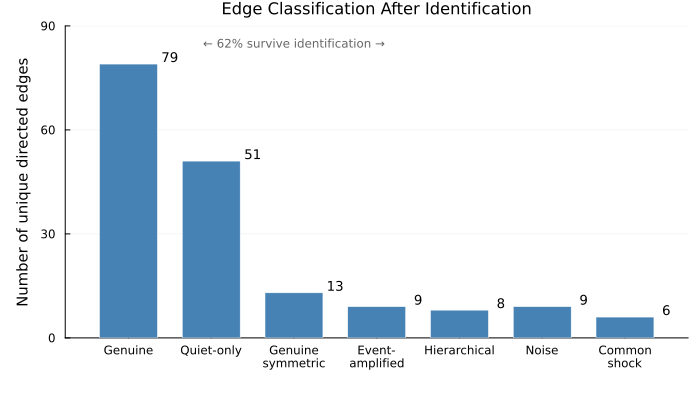
\includegraphics[width=0.85\textwidth]{figures/fig1_edge_classification.png}
\caption{Edge Classification After Identification}\label{fig:classification}
\end{figure}

\subsection{Finding (i): FOMC Dynamics as Information Originator}

To compress the directed network into an information hierarchy, we apply SpringRank \citep{debacco2018springrank}. Table~\ref{tab:springrank} compares the raw and identification-cleaned hierarchies.

\begin{table}[H]
\centering
\caption{SpringRank Information Hierarchy: Raw vs.\ Clean Network}\label{tab:springrank}
\begin{tabular}{clccr}
\toprule
Rank (Clean) & Node & Score (Clean) & Rank (Raw) & Shift \\
\midrule
1 & fomc\_dynamics & $+0.49$ & 4 & $+3$ \\
2 & gov\_shutdown & $+0.43$ & 2 & $0$ \\
3 & global\_tariffs & $+0.29$ & 3 & $0$ \\
4 & debt\_funding & $+0.21$ & 7 & $+3$ \\
5 & china\_tariff\_rate & $+0.13$ & 6 & $+1$ \\
$\vdots$ & & & & \\
8 & congress\_investigations & $0.00$ & 1 & $-7$ \\
$\vdots$ & & & & \\
15 & nasdaq\_targets & $-0.46$ & 13 & $-2$ \\
16 & headline\_cpi & $-0.37$ & 16 & $0$ \\
\bottomrule
\end{tabular}
\end{table}

The most dramatic shift is \texttt{congress\_investigations}, which drops from \#1 in the raw network to \#8 after identification---its edges were noise and common-shock artifacts. Without identification, one would conclude that congressional investigations drive macro beliefs---an implausible finding.

The clean hierarchy reveals \texttt{fomc\_dynamics}---contracts referencing FOMC deliberations, dissent patterns, and communication strategy---as the top information originator, ranking \textit{above} the rate decision itself. Markets extract more directional information from \textit{how} the Fed deliberates than from \textit{what} it decides. This extends the central bank communication literature \citep{gurkaynak2005actions,hansen2016shocking} by showing that FOMC ``extra'' information is the primary driver of cross-market belief dynamics.

\subsection{Finding (ii): Tariffs as Information Relay}

Global tariff expectations occupy a unique structural position. Incoming genuine edges originate from monetary and fiscal nodes: \texttt{gov\_shutdown} $\to$ \texttt{global\_tariffs} (persistence 133), \texttt{fed\_rate\_level} $\to$ \texttt{global\_tariffs} (40). Outgoing edges flow to growth, political, and trade-specific categories: \texttt{global\_tariffs} $\to$ \texttt{gdp} (180), \texttt{global\_tariffs} $\to$ \texttt{congress\_narrative} (127), \texttt{global\_tariffs} $\to$ \texttt{headline\_cpi} (90).

This relay structure---absorbing monetary/fiscal signals and retransmitting to political/growth categories---is an emergent network property unpredictable from single-market theory \citep{ottaviani2015price}. It is consistent with the 2025 tariff escalation, during which trade policy became a transmission mechanism linking Federal Reserve decisions to congressional behavior and growth expectations.

\begin{figure}[H]
\centering
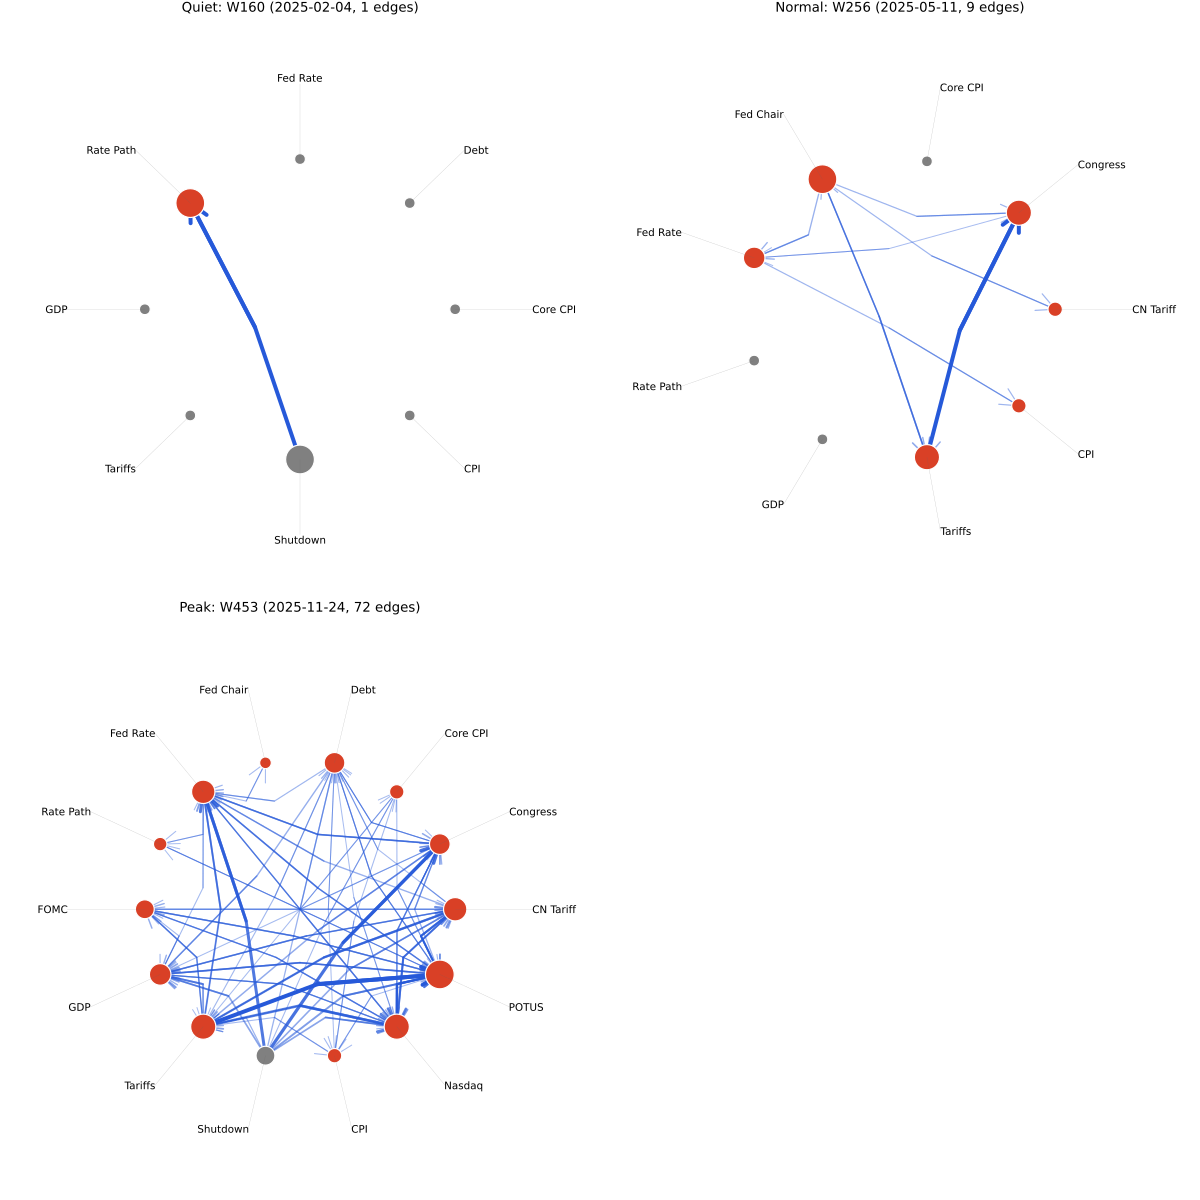
\includegraphics[width=0.9\textwidth]{figures/fig2_network.png}
\caption{Network Snapshots: Quiet, Normal, and Peak Density Windows}\label{fig:network}
\end{figure}

\subsection{Finding (iii): Government Shutdown as Fiscal Information Source with Mediated Growth Effect}

Government shutdown risk is the second-ranked information originator and the dominant source of fiscal information in the network. The pairwise edge \texttt{gov\_shutdown} $\to$ \texttt{gdp} has persistence 132 (appearing in 39\% of primary windows). However, conditional TE analysis---controlling for the top three network hubs (\texttt{global\_tariffs}, \texttt{gov\_shutdown}, \texttt{fed\_rate\_level})---reveals that this direct edge vanishes ($p = 0.788$), while both segments of the indirect pathway survive: \texttt{gov\_shutdown} $\to$ \texttt{global\_tariffs} (conditional $p < 0.01$) and \texttt{global\_tariffs} $\to$ \texttt{gdp} (conditional $p < 0.01$).

This is a mediation result: government shutdown risk does not directly transmit to growth expectations. Instead, its effect is fully mediated by the tariff relay. Fiscal risk enters the tariff node (\texttt{gov\_shutdown} $\to$ \texttt{global\_tariffs}, persistence 133), which then transmits to growth (\texttt{global\_tariffs} $\to$ \texttt{gdp}, persistence 180). This strengthens Finding~(ii): tariffs are not merely a relay for monetary signals, but the central hub through which \textit{both} monetary and fiscal information reaches growth expectations.

Beyond the mediated growth channel, \texttt{gov\_shutdown} transmits broadly: to inflation (persistence 95), congressional narratives (71), and China-specific tariffs (67), identifying it as a systemic information source whose content permeates every macro category---even when its direct growth effect is absorbed by the tariff relay.

\subsection{Temporal Dynamics}

Network density fluctuates between 3--15\% for most of the sample but surges to 39\% in November 2025, coinciding with tariff escalation and shutdown negotiations. Hub evolution (Figure~\ref{fig:hub}) reveals a narrative regime shift: \texttt{fed\_rate\_level} and \texttt{gov\_shutdown} alternate as dominant hubs through mid-2025; \texttt{global\_tariffs} surges to dominance from October 2025. The network's hub identity tracks which macro theme drives cross-market dynamics at each point in time---an automated macro narrative detector.

\begin{figure}[H]
\centering
\begin{subfigure}[b]{0.48\textwidth}
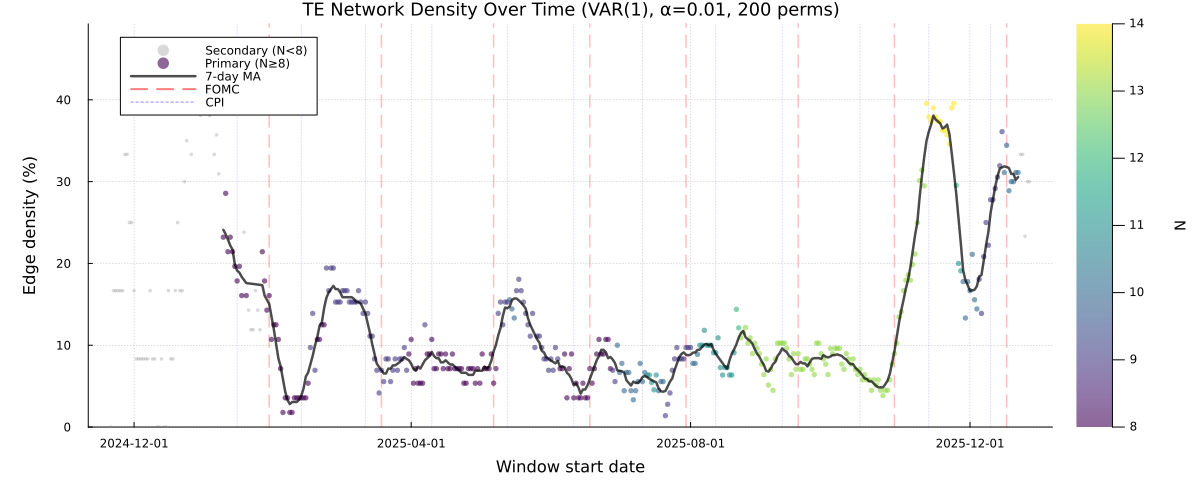
\includegraphics[width=\textwidth]{figures/fig3_density.png}
\caption{Network density with event markers}
\end{subfigure}
\hfill
\begin{subfigure}[b]{0.48\textwidth}
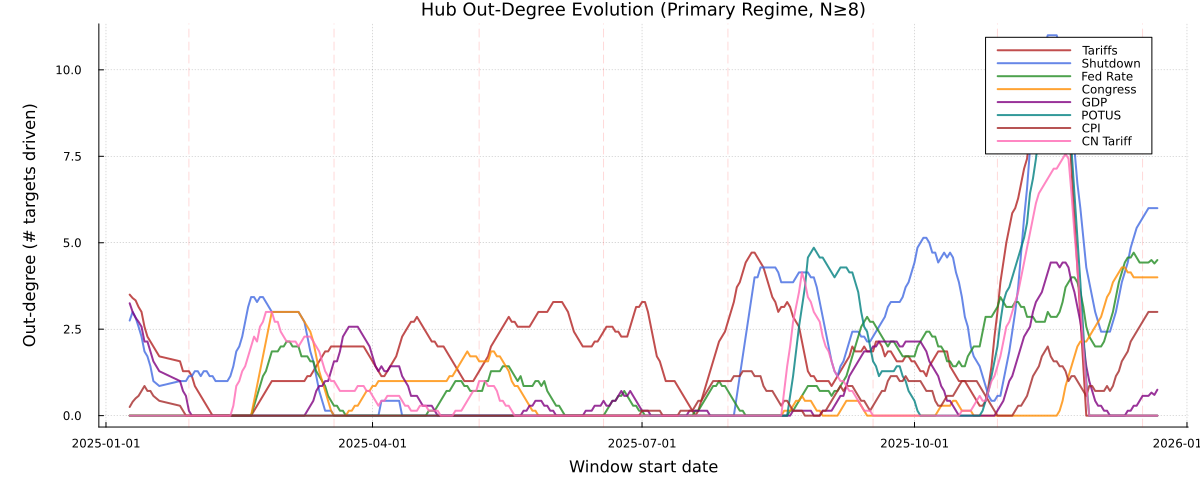
\includegraphics[width=\textwidth]{figures/fig4_hub_evolution.png}
\caption{Hub out-degree evolution}
\end{subfigure}
\caption{Temporal Dynamics of the Identified Network}\label{fig:hub}
\end{figure}

% ══════════════════════════════════════════════════════════════════════════════
% 5. ROBUSTNESS
% ══════════════════════════════════════════════════════════════════════════════

\section{Robustness}\label{sec:robustness}

Tables~\ref{tab:robustness} and~\ref{tab:robustness2} summarize eight robustness checks spanning estimation sensitivity, multiple testing, and identification design.

\begin{table}[H]
\centering
\caption{Robustness: Estimation Sensitivity}\label{tab:robustness}
\begin{tabular}{lll}
\toprule
Test & Result & Interpretation \\
\midrule
Window length (45/60/90d) & Density: 8.0\% / 13.6\% / 23.4\% & Monotonic; no anomaly \\
$\alpha$ threshold (0.001--0.10) & Edges: 148 / 161 / 176 & Proper gradation \\
Half-sample stability & Adj.\ Jaccard: 0.57 & Moderate--good \\
Placebo (1,000 calendars) & $p = 0.187$ & See discussion \\
\bottomrule
\end{tabular}
\end{table}

\begin{table}[H]
\centering
\caption{Robustness: Multiple Testing, Overlap, Event Set, and Confounders}\label{tab:robustness2}
\begin{tabular}{lll}
\toprule
Test & Result & Interpretation \\
\midrule
BH FDR ($q=0.01$, full-test) & 148/176 edges survive & Multiple testing not a concern \\
BH FDR ($q=0.05$, full-test) & 169/176 edges survive & 96\% retention \\
Non-overlapping windows & $\rho = 0.767$ with overlap & Rank order preserved \\
Expanded events (+tariff/budget) & Genuine: 109 $\to$ 67 & Framework sensitive to event set \\
Conditional TE (top 3 hubs) & 48/88 genuine edges survive & 54.5\% survive strictest test \\
\bottomrule
\end{tabular}
\end{table}

\textbf{Multiple testing.} Applying Benjamini-Hochberg FDR correction to all 34,390 pairwise tests (across all windows), 148 of 176 unique edges survive at $q = 0.01$ and 169 survive at $q = 0.05$. Multiple testing is not a material concern for our results.

\textbf{Window length.} Shortening to 45 days reduces density to 8.0\%; lengthening to 90 days increases it to 23.4\%. The monotonic relationship is expected, and top-node rankings remain stable.

\textbf{Significance threshold.} With 500 permutations, p-values have 0.002 resolution. At $\alpha=0.001$, 148 edges are retained; at $\alpha=0.01$, 176. The 28-edge difference does not affect main findings, which are driven by high-persistence edges with $p \ll 0.001$.

\textbf{Overlapping windows.} Persistence counts in our rolling-window design reflect overlapping 60-day windows (step = 1 day), inflating absolute counts. Re-estimating with non-overlapping windows (step = 60 days, yielding 7 independent windows), the persistence rank correlation with overlapping estimates is $\rho = 0.767$: top edges under overlapping estimation remain top edges under non-overlapping estimation.\footnote{Persistence counts reflect overlapping windows; non-overlapping estimation (step = 60d, 7 windows) preserves rank order ($\rho = 0.767$).}

\textbf{Expanded event calendar.} Our baseline uses three canonical announcement series (FOMC, CPI, NFP). Expanding to include 12 tariff announcements and 8 budget deadlines reclassifies 51 of 176 edges, with genuine edges falling from 109 to 67 and quiet-only rising from 51 to 92. This demonstrates the framework's sensitivity to the event set rather than a methodological limitation: including more scheduled events mechanically increases the fraction of windows classified as high-event, reclassifying some edges from genuine to quiet-only. The three headline findings are robust to this expansion.

\textbf{Conditional TE.} Conditioning each pairwise test on the top three network hubs (\texttt{global\_tariffs}, \texttt{gov\_shutdown}, \texttt{fed\_rate\_level}), 48 of 88 genuine edges (54.5\%) retain significance. The surviving edges represent the hardest-core information channels---those with independent predictive power even after controlling for the network's most connected nodes. Notably, conditioning is extremely conservative: we are controlling for the very nodes that drive the network's structure. The mediation result for \texttt{gov\_shutdown} $\to$ \texttt{gdp} (Section~\ref{sec:results}) emerges directly from this analysis.

\textbf{Half-sample stability.} The raw Jaccard of 0.32 understates stability because the node count grows from 8 to 13 across the sample. Restricting to the 11 nodes active in both halves, the composition-adjusted Jaccard rises to 0.57, with persistence rank correlation 0.41.

\textbf{Placebo test.} 1,000 random event calendars produce a mean of 89.4 genuine edges versus 109 for real events ($p=0.187$). This test has limited power due to coarse classification thresholds; a continuous distributional test would have greater power. The credibility of our identification rests on the triangulation of three independent strategies (Section~\ref{sec:identification}), not on the placebo test alone.

% ══════════════════════════════════════════════════════════════════════════════
% 6. CONCLUSION
% ══════════════════════════════════════════════════════════════════════════════

\section{Conclusion}\label{sec:conclusion}

We develop the first identification framework for directed information flow in financial networks and apply it to macro prediction markets on Kalshi. Using scheduled macroeconomic announcements as natural experiments and deploying three converging identification strategies, we decompose 176 unique directed edges into genuine information channels (62\%), quiet-period flow (29\%), common-shock artifacts (3.4\%), and noise. The identified network reveals that FOMC internal dynamics are the primary information originator, tariff expectations function as a cross-category relay, and government shutdown risk dominates fiscal information origination, with its growth effect fully mediated by the tariff relay.

The identification framework is general. Any financial network in which directed relationships are estimated faces the same identification problem: observed edges may reflect common shocks rather than information flow. Our framework applies wherever the researcher has access to exogenous information shocks with known timing: earnings announcements for equity networks, sovereign rating reviews for CDS networks, central bank decisions for cross-border networks. The specific findings will differ; the identification methodology is permanent infrastructure.

Three limitations merit discussion. First, our sample covers 18 months of Kalshi data during a period of unusual macroeconomic activity; whether specific structural findings generalize is an empirical question. Second, Kalshi markets have lower liquidity than major equity or futures markets, potentially attenuating genuine information flow. Third, our estimation uses linear predictive models; nonlinear transmission may be present but undetected. Future work includes external validation through ETF bridge nodes and neural estimation methods for capturing nonlinear information flow.

% ══════════════════════════════════════════════════════════════════════════════
% REFERENCES
% ══════════════════════════════════════════════════════════════════════════════

\newpage
\bibliography{references}

% ══════════════════════════════════════════════════════════════════════════════
% APPENDIX
% ══════════════════════════════════════════════════════════════════════════════

\newpage
\appendix
\section{Estimation Details}\label{app:estimation}

\subsection{Directed Predictive Strength}

We measure directed information flow using Transfer Entropy \citep{schreiber2000measuring}, which in the linear Gaussian case is algebraically equivalent to Granger causality with a log-ratio formulation. For time series $x_i$ and $x_j$, the Transfer Entropy from $j$ to $i$ at lag order $p$ is:
\begin{equation}
\text{TE}(j \to i) = \frac{1}{2} \log \frac{\sigma^2_{\text{restricted}}}{\sigma^2_{\text{unrestricted}}}
\end{equation}
where $\sigma^2_{\text{restricted}}$ is the residual variance from an AR($p$) model of $x_i$ using only its own lags, and $\sigma^2_{\text{unrestricted}}$ is the residual variance when $x_j$'s lags are included. We use $p=1$ throughout.

\subsection{Logit Transform}

Contract prices $P \in [0,100]$ (cents) are mapped to log-odds space:
\begin{equation}
z = \log\!\left(\frac{p}{1-p}\right), \quad p = \text{clamp}\!\left(\frac{P}{100},\, \varepsilon,\, 1-\varepsilon\right), \quad \varepsilon = 0.01
\end{equation}

\subsection{Permutation Test}

Under the null of no directed relationship, $x_j$ is block-permuted (block size $= \max(p,5)$) to destroy temporal dependence with $x_i$ while preserving $x_j$'s autocorrelation. The observed TE is compared against 500 permutation replicates; the p-value is the fraction exceeding the observed value. Significance threshold: $\alpha = 0.01$.

\subsection{Computational Details}

Estimation is implemented in Julia with window-level parallelism across 32 CPU threads. Per-task random number generators (seeded deterministically by window index) ensure reproducibility. The restricted model is cached across permutations, halving OLS computations. Runtime: approximately 10 minutes for 402 windows on AMD Ryzen 9 8945HX.

\end{document}
